\input{lib/dissertationelse.tex}
\input{lib/dissertationexclude.tex}
\input{lib/dissertationonly.tex}

\begin{figure*}

\begin{subfigure}{0.425\linewidth}
\centering

\includegraphics[width=\linewidth,trim=0 0.2cm 0 0,clip]{../binder/binder-bucket=prq49--a=all_stints_all_series_profiles+endeavor=16--fitness_complexity.ipynb/binder/teeplots/bucket=prq49--a=all_stints_all_series_profiles+endeavor=16--fitness_complexity/annot=morph+hue=series+viz=lineplot+what=16005+x=stint+y=flagged-advantageous-sites+ext=.pdf}

\vspace{-1ex}

\caption{\footnotesize genotype complexity, case study (blue) vs. others}
\label{fig:16005-timelapse:genotype-complexity}
\end{subfigure}%
\begin{subfigure}{0.425\linewidth}
\centering

\includegraphics[width=\linewidth,trim=0 0.2cm 0 0,clip]{../binder/binder-bucket=prq49--a=all_stints_all_series_profiles+endeavor=16--interface_complexity.ipynb/binder/teeplots/bucket=prq49--a=all_stints_all_series_profiles+endeavor=16--interface_complexity/annot=morph+hue=series+viz=lineplot+what=16005+x=stint+y=cardinal-interface-complexity+ext=.pdf}

\vspace{-1ex}

\caption{\footnotesize phenotype complexity, case study (blue) vs. others}
\label{fig:16005-timelapse:phenotype-complexity}
\end{subfigure}%
\begin{subfigure}{0.15\linewidth}
\centering

\includegraphics[width=\linewidth,trim=1cm 0.15cm 0.8cm 0,clip]{../binder/binder-bucket=prq49--a=all_stints_all_series_profiles+endeavor=16--fitness_complexity.ipynb/binder/teeplots/bucket=prq49--a=all_stints_all_series_profiles+endeavor=16--fitness_complexity/how=mean+hue=series+inner=box+iqr=shade+viz=scatterplot+what=16005+x=flagged-advantageous-sites+y=cardinal-interface-complexity+ext=.pdf}

\vspace{-1ex}

\caption{\footnotesize mean g.c./p.c.}
\label{fig:16005-timelapse:mean-complexity}
\end{subfigure}

\begin{tcolorbox}[
  enhanced,
  colframe=morphj!30!white,
  colback=morphj!4!white,
  boxrule=0.8pt,
  arc=1pt,
  boxsep=0pt,
  left=0pt,right=0pt,top=0pt,bottom=0pt,
  width=\linewidth,
]
\savebox{\morphjtitlebox}{%
  \begin{tabular}{@{}c@{}}
    \bfseries\footnotesize morph~\tikz[baseline=(morphjbadge.base)]{%
      \node[draw=black,very thick,fill=morphj,circle,inner sep=1pt,minimum size=1.1em,text=white] (morphjbadge) {$\boldsymbol{j}$};%
    }\\[2pt]
    \bfseries\footnotesize life history\\[3pt]
    \scriptsize video animation:\\[-2pt]
    \scriptsize\href{https://hopth.us/hr}{\texttt{\scriptsize hopth.us/hr}}
  \end{tabular}%
}
% each of the 5 panels is 0.2\panelcolwd wide and holds a picture set at
% 0.9 of that, so 0.01\panelcolwd of slack already sits at the column's
% outer edge; leading the panel row with the same amount gives the frame
% the same clearance on top and right
\setlength{\panelcolwd}{\dimexpr\linewidth-\wd\morphjtitlebox-12pt\relax}
\setlength{\panelpad}{0.01\panelcolwd}
% The pictures are cropped, so how tall they come out is not something to
% assume; set one and measure it.
\savebox{\panelimgbox}{%
  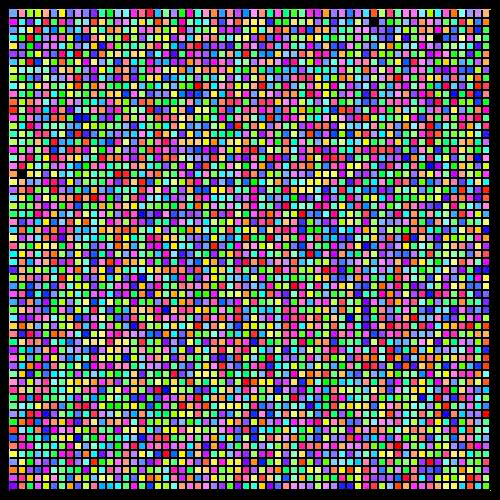
\includegraphics[width=0.18\panelcolwd,trim=4cm 4cm 4cm 4cm,clip]{img/a=kin-group-id+idx=0+proc=0+series=16005+stint=100+thread=0+update=16-8752_16/frame_0001.png}%
}
\setlength{\panelimght}{\dimexpr\ht\panelimgbox+\dp\panelimgbox\relax}
% a specimen subcaption, twice: strutted, to measure the line it is set
% on, and bare, to measure how far its letters actually reach.
% The difference is the slack the line leaves over and under them, which
% counts towards the white space the reader sees.
\savebox{\panelcapbox}{\footnotesize\strut(h) update 952}
\savebox{\panelcapinkbox}{\footnotesize(h) update 952}
% A probe panel: the same picture captioned the same way, but unnumbered,
% so it steps no counter and writes no list-of-figures entry.
% What it holds beyond the picture and that line is the skip the caption
% package leaves above a subcaption, which differs between TeX
% distributions --- so the figure tightens it by proportion below rather
% than replacing it with a length of its own.
\savebox{\panelprobebox}{%
  \begin{subfigure}{0.2\panelcolwd}
  \centering
  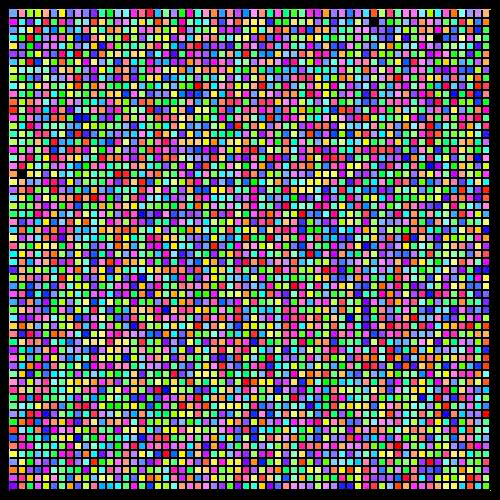
\includegraphics[width=0.9\linewidth,trim=4cm 4cm 4cm 4cm,clip]{img/a=kin-group-id+idx=0+proc=0+series=16005+stint=100+thread=0+update=16-8752_16/frame_0001.png}%
  \caption*{update 8}
  \end{subfigure}%
}
\setlength{\panelcapskip}{\dimexpr\ht\panelprobebox+\dp\panelprobebox
  -\panelimght-\ht\panelcapbox-\dp\panelcapbox\relax}
% the white space actually on show above and below a subcaption
\setlength{\panelcapabove}{\dimexpr\panelcapskip
  +\ht\panelcapbox-\ht\panelcapinkbox\relax}
\setlength{\panelcapbelow}{\dimexpr\panelcapskip
  +\dp\panelcapbox-\dp\panelcapinkbox\relax}
% take a third off the gap above the subcaptions and half off the gap
% below them, both measured as seen
\setlength{\panelcaptrim}{0.33\panelcapabove}
\setlength{\panelcappad}{0.5\panelcapbelow}
\addtolength{\panelcappad}{\dimexpr\dp\panelcapinkbox-\dp\panelcapbox\relax}
% Save the panel row so its height is measured rather than derived from
% lengths that vary between TeX distributions.
\savebox{\panelrowbox}{%
\begin{subfigure}{0.2\panelcolwd}
\centering
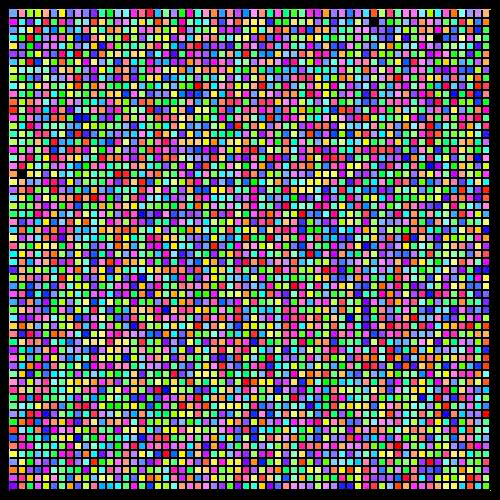
\includegraphics[width=0.9\linewidth,trim=4cm 4cm 4cm 4cm,clip]{img/a=kin-group-id+idx=0+proc=0+series=16005+stint=100+thread=0+update=16-8752_16/frame_0001.png}%
\vspace{-\panelcaptrim}%
\caption{update 8}
\label{fig:16005-timelapse:update64}
\end{subfigure}%
\begin{subfigure}{0.2\panelcolwd}
\centering
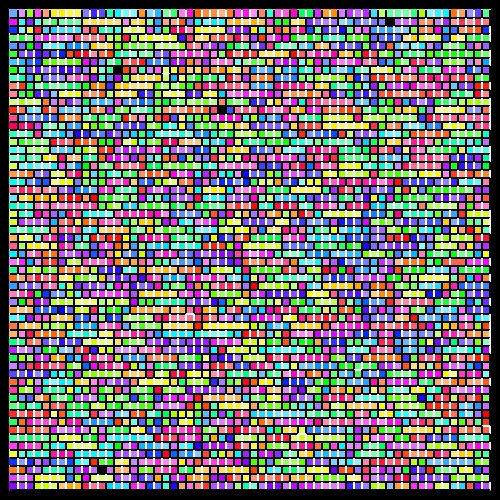
\includegraphics[width=0.9\linewidth,trim=4cm 4cm 4cm 4cm,clip]{img/a=kin-group-id+idx=0+proc=0+series=16005+stint=100+thread=0+update=16-8752_16/frame_0016.png}%
\footnotesize
\vspace{-\panelcaptrim}%
\caption{update 32}
\label{fig:16005-timelapse:update256}
\end{subfigure}%
\begin{subfigure}{0.2\panelcolwd}
\centering
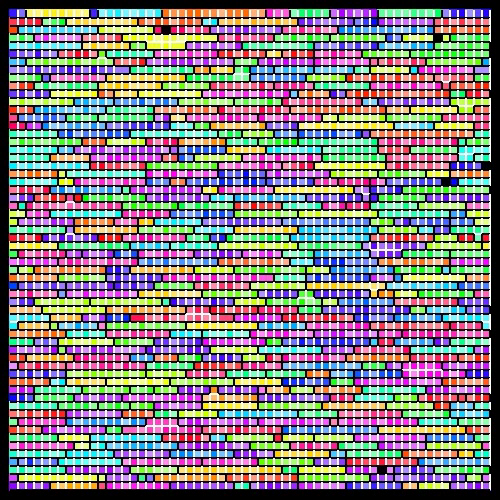
\includegraphics[width=0.9\linewidth,trim=4cm 4cm 4cm 4cm,clip]{img/a=kin-group-id+idx=0+proc=0+series=16005+stint=100+thread=0+update=16-8752_16/frame_0052.png}%
\footnotesize
\vspace{-\panelcaptrim}%
\caption{update 104}
\label{fig:16005-timelapse:update832}
\end{subfigure}%
\begin{subfigure}{0.2\panelcolwd}
\centering
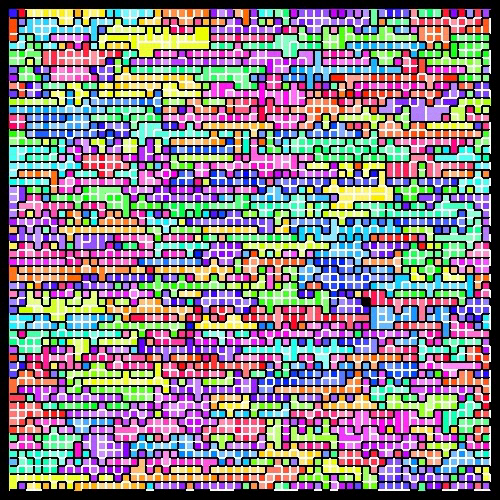
\includegraphics[width=0.9\linewidth,trim=4cm 4cm 4cm 4cm,clip]{img/a=kin-group-id+idx=0+proc=0+series=16005+stint=100+thread=0+update=16-8752_16/frame_0420.png}%
\footnotesize
\vspace{-\panelcaptrim}%
\caption{update 840}
\label{fig:16005-timelapse:update6720}
\end{subfigure}%
\begin{subfigure}{0.2\panelcolwd}
\centering
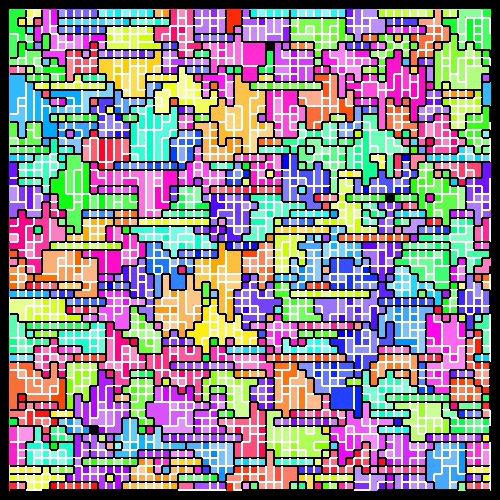
\includegraphics[width=0.9\linewidth,trim=4cm 4cm 4cm 4cm,clip]{img/a=kin-group-id+idx=0+proc=0+series=16005+stint=100+thread=0+update=16-8752_16/frame_0476.png}%
\footnotesize
\vspace{-\panelcaptrim}%
\caption{update 952}
\label{fig:16005-timelapse:update7616}
\end{subfigure}%
}
\setlength{\panelrowht}{\dimexpr\panelpad+\ht\panelrowbox+\dp\panelrowbox
  +\panelcappad\relax}
\setlength{\tabcolsep}{0pt}
\renewcommand{\arraystretch}{1}
\begin{tabular}{@{}>{\cellcolor{morphj!25!white}}m{\dimexpr\wd\morphjtitlebox+8pt\relax}@{\hspace{4pt}}m{\panelcolwd}@{}}
% Both cells are boxes of the same measured height, so they line up top
% and bottom whatever the surrounding lengths happen to be; the title
% then centers on the pictures by sitting in a box exactly as tall as
% they are.
\parbox[c][\panelrowht][t]{\dimexpr\wd\morphjtitlebox+8pt\relax}{%
  \vspace*{\panelpad}%
  \vbox to \panelimght{%
    \vfil
    \hbox to \linewidth{\hfil\usebox{\morphjtitlebox}\hfil}%
    \vfil
  }%
}
&
\parbox[c][\panelrowht][t]{\panelcolwd}{%
  \vspace*{\panelpad}%
  \usebox{\panelrowbox}%
}
\\
\end{tabular}

\end{tcolorbox}

\vspace{-1.5ex}

\caption{%
\textbf{Case study strain.}
\footnotesize
Compared to other replicates, case study 16005 sustained extreme outlying complexity (upper panels \labelcref{fig:16005-timelapse:genotype-complexity,fig:16005-timelapse:phenotype-complexity,fig:16005-timelapse:mean-complexity}) and exhibited unique multi-stage patterned growth (lower panels \labelcref{fig:16005-timelapse:update64,fig:16005-timelapse:update256,fig:16005-timelapse:update832,fig:16005-timelapse:update6720,fig:16005-timelapse:update7616}).
Genotype complexity counts genome sites contributing to fitness; phenotype complexity counts distinct cell input/output operations contributing to fitness --- both determined via knockout/interference trials.
Snapshots show example life history (morph ``$j$,'' transfer round 100; Supplementary Table \ref{tab:morph_descriptions}).
Hue denotes, and black borders divide, multicell groups; white borders reflect inner structure.
From initial unicell groups (\ref{fig:16005-timelapse:update64}), cells replicate to form horizontal ``cigar-like'' bodies (\labelcref{fig:16005-timelapse:update256,fig:16005-timelapse:update832}).
In a delayed second stage of growth, groups expand vertically to produce a ``box-like'' final morphology (\labelcref{fig:16005-timelapse:update6720,fig:16005-timelapse:update7616}).
During this secondary phase of growth, some groups establish cigar-like propagules (\labelcref{fig:16005-timelapse:update7616}).
}
\label{fig:16005-timelapse}

\end{figure*}


\section{Results}

Our investigation begins by dissecting how a particularly complex multicellular life history arose in a case study evolutionary trial (Sections \labelcref{sec:case-study-lineage,sec:biotic-context-influences-fitness,sec:case-study-strain-produces-biotic-selection,sec:self-acting-selection-maintains-complexity-in-case-study-strain}).
Then, motivated by this case study, we test how biotic selection effects influence evolved complexity across evolutionary trials (Sections \labelcref{sec:biotic-selection-drives-multicell-complexity,sec:biotic-selection-acts-between-coevolving-lineages}).

\subsection{Case-study Lineage}
\label{sec:case-study-lineage}

To screen structural and functional complexity across evolutionary replicates, we isolated distinct adaptations via genetic knockout and phenotypic interference competitions (Figures \labelcref{fig:16005-timelapse:genotype-complexity,fig:16005-timelapse:phenotype-complexity}, Section \ref{sec:measuringcomplexity}).
Among 40 replicates, an extreme outlier in genotype and phenotype complexity sustained excess of 3$\times$ IQR in both dimensions (blue highlight, Figure \ref{fig:16005-timelapse:mean-complexity}).

Closer examination revealed this lineage to exhibit unique patterned growth and multi-stage life history.
Growing from unicellular inoculum (Figure \labelcref{fig:16005-timelapse:update64}), group bodies first elongate horizontally to establish an asymmetrical ``cigar-like'' morphology (Figure \labelcref{fig:16005-timelapse:update256,fig:16005-timelapse:update832}).
Then, in a secondary phase of growth, groups expand in the vertical direction to establish an irregular ``box-like'' morphology (Figure \labelcref{fig:16005-timelapse:update6720,fig:16005-timelapse:update7616}).

To investigate how complexity arose and stabilized in this lineage, we examined its history in detail as a case study --- reported next.

\input{fig/keyfig.tex}

\subsubsection{Morphology}

Qualitative categorization of morphologies sampled across each of 100 evolutionary passages
% Supplementary Table \ref{tab:morph_descriptions} provides more detailed descriptions of each qualitative morph category, as well as a video and still image example of each.
% Supplementary Table \ref{tab:morph_by_stint} provides morph categorization for each transfer round as well as links to view the transfer round's specimen in a video or in-browser web simulation.
identified nine classes: labeled ``$b$'' through ``$j$'' (Figure \ref{fig:keyfig:morph}, Supplementary Tables \labelcref{tab:morph_descriptions,tab:morph_by_stint}, and Supplementary Figure \ref{fig:phylo_parsimony_tree}).
\unskip\footnote{%
Descriptions of morphs $c$, $d$, $f$, $h$, and $i$ --- which were sampled rarely --- appear in supplementary material.
Morph $a$ was assigned to an independent short-lived lineage.
}

Early sampled genomes mostly grew as unicells and small groups up to 4 cells (morph $b$).
%, although our earliest sample from the case study lineage formed oversized groups through unchecked cell proliferation (morph $c$, transfer round 2).

The case study lineage's cigar-like patterning first arose at transfer round 15 (morph $e$) and
% Earlier, at transfer round 14, we also saw large group formation (morph $d$, irregular clumps of 10 to 15 cells), but the sample's lineage appears to have subsequently gone extinct.
secondary box-like vertical growth first arose at transfer round 45 (morph $g$).
% However, around transfer round 60, cigar-like morph $e$ began to be sampled as a reversion from morph $g$.
Finally, at transfer round 100, we first observed morph $j$ (panels \labelcref{fig:16005-timelapse:update64,fig:16005-timelapse:update256,fig:16005-timelapse:update832,fig:16005-timelapse:update6720,fig:16005-timelapse:update7616}), which began to produce cigar-like daughter propagules during the secondary growth phase.

\subsubsection{Complexity}

After cataloging morphology, we next sought to characterize its relationship to measures of structural and functional complexity.
We thus conducted additional knockout and interference trials to assay genotype and phenotype complexity of samples from each transfer round (Figure \labelcref{fig:keyfig:gcomplexity,fig:keyfig:pcomplexity}, Supplementary Figure \ref{fig:complexity}).

In several instances, complexity measures increased abruptly with new morphology.
For instance, at transfer round 14, morph $d$ (irregular clumps of 10 to 15 cells) coincided with a spike in genotype complexity from 28 to 44 sites.
At transfer round 15, cigar-like morph $e$ grew phenotype complexity over threefold from 5 to 17 interactions.
However, in contrast to these abrupt innovations, genotype complexity grew in a more gradual phase after the rise of cigar-like morph $e$ from 27 to 55 sites between transfer rounds 16 and 39.

% In two independent sublineages --- both going extinct --- genotype and phenotype complexity simultaneously and abruptly crashed near zero.
% Both were morph $i$: unrestricted cell proliferation with small irregular groups.
% No complexity crash, however, appears in assays configured with biotic background --- suggesting a contingent dependency to this background may have developed (Supplementary Figure \ref{fig:DOTO}).

% https://github.com/mmore500/oee4/blob/binder-2025-11-30-genome-complexity-regression.ipynb/binder/2025-11-30-genome-complexity-regression.ipynb
Split regression analysis suggests genotype complexity developed in two distinct regimes (Davies test, $p < 10^{-14}$, adj. $R^2=0.43$): increasing until transfer round 34 (Wald test, $R^2 = 0.59$, $p < 10^{-6}$), and then decreasing (Wald test, $R^2 = 0.24$, $p < 10^{-4}$) (Supplementary Figure \ref{fig:complexity-cryptic-regression:split}) --- likely due to gains in mutational robustness masking knockout sensitivity (Supplementary Section \ref{sec:supp-genotype-complexity}).
% Thus, the evolutionary trajectory of genotype complexity appears to be initial growth followed by stabilization.

\subsubsection{Adaptation}

Next, we examined fitness change along the case study lineage.
For this purpose, we competed successive samples to test for fitness gains at each step.
Across 100 assays, 57 sampled genotypes outcompeted their predecessor by a significant margin (Figure \ref{fig:keyfig:morph}, Supplementary Figures \labelcref{fig:median_fitness_differential_symlog,fig:fitness_gain_or_loss}).
Fitness gains became more sparse at later timepoints --- a notable exception, though, being strong fitness gain with 500-site genome expansion at transfer round 93 (Figure \ref{fig:keyfig}).
% Fitness differentials during the first 40 transfer rounds are generally higher magnitude than later fitness differentials, although a strong fitness differential occurs at transfer round 93 coincident with a genome duplication.

Besides the 57 adaptive steps discussed above, 23 steps were neutral and --- surprisingly --- 20 were deleterious (Figure \ref{fig:keyfig:morph}).
To assess whether these apparent fitness losses could be explained by within-population variation, we repeated assays to compete whole-population samples rather than monoclonal isolates.
However, whole-population competition results remained similar: 50 steps were adaptive, 34 neutral, and 16 deleterious (Supplementary Figure \ref{fig:keyfig-Prefatory}).

Although rarer than fitness gains ($p < 10^{-4}$; exact Binomial test), nearly one in five lineage intermediates thus appeared maladaptive.
While drift effects can produce such maladaptation (carrying capacity supported only around 500 cigar-like multicell groups), it could also stem from trade-offs imposed by co-evolving ecological context \citep{brady2019causes} --- a possibility we investigate next.

\subsection{Adaptation to Co-evolved Ecological Context}

Experimental design maintained long-term coexistence of an additional independent lineage alongside the case study strain (Section \ref{sec:methods}).
To test whether selection imposed by this ``background'' strain could explain seeming maladaptations, we repeated fitness competitions to incorporate co-evolved biotic context (see Figure \ref{fig:fit:bbg}).
% \unskip\footnote{%
% For this purpose, we used genomes collected from the co-evolved lineage at ``prefatory'' transfer round $n$, rather than $n + 1$.
% Results using co-evolved genomes from ``contemporary'' transfer round $n + 1$ were generally similar, and are included in supplementary material.
% }

In co-evolved context, whole-population maladaptations decreased from 16 to 3 (Supplementary Figure \ref{fig:sign-change-prefatory-population}).
Lower assay sensitivity might partially explain this result (no detected effect in 52 vs. 23 cases).
However, 6 cases did evidence sign-change effects: where fitness losses became fitness gains in co-evolved context.
% We saw no instances of the reverse, as all 3 outcomes deleterious in ecological context were also deleterious without it.

Thus, having found biotic context to exert selection on the case study strain, we next set out to test how such ecological interactions influenced its evolved complexity.

\subsection{Biotic Context Influences Fitness}
\label{sec:biotic-context-influences-fitness}

\begin{figure}
\centering
\captionsetup[subfigure]{font=footnotesize,skip=0pt}

\begin{subfigure}[t]{0.696\linewidth}
\centering

\includegraphics[width=\linewidth, trim=0.8cm 0 0 0, clip]{../binder/binder-2025-11-30-external-selfbb-truebb.ipynb/binder/teeplots/2025-11-30-external-selfbb-truebb/hue=kind1+style=kind1+viz=lineplot+x=competition-stint+y=focal-prevalence+ext=.pdf}
\caption{transfer rounds 0 to 100}
\label{fig:fitness-background:timeseries}
\end{subfigure}%
\begin{subfigure}[t]{0.304\linewidth}
\centering

\includegraphics[width=\linewidth, trim=1.3cm 0 0 0.1cm, clip]{../binder/binder-2025-11-30-external-selfbb-truebb.ipynb/binder/teeplots/2025-11-30-external-selfbb-truebb/hue=kind+inner=quartile+viz=violinplot+x=kind+y=focal-prevalence+ext=.pdf}
\caption{rounds 15 to 100}
\label{fig:fitness-background:distribution}
\end{subfigure}

\caption{%
\textbf{Patterned growth creates biogenic niche.}
\footnotesize
Around transfer round 15, fitness of case study strain in self-context diverges significantly above other contexts.
For background type ``None,'' competition is initialized 50\%/50\% between compared strains (Figure \ref{fig:fit:nobbg}).
Otherwise, competition is initialized 25\%/25\%/50\% between compared strains and background (Figure \ref{fig:fit:bbg}).
Shaded bands are bootstrap 95\% CI.
Mann-Whitney test with Cliff's $\delta$ reported.
% From this point onwards, self context affords significantly higher tournament fitness than ecological context (Mann-Whitney $U$ test, $p<10^{-25}$).
% By contrast, ecological context more closely tracks background-free tournament fitness, though exhibiting strong episodic deviations.
% Absent background context, the case study strain's tournament fitness fell below null expectation of 0.5 ($\mu=0.39$; $[0.31,\;0.43]$ bootstrap 95\% CI, $n=40$).
% By contrast, in self-context tournament fitness fell above null expectation ($\mu=0.72$; $[0.69,\;0.76]$ bootstrap 95\% CI, $n=40$).
}
\label{fig:fitness-background}
\end{figure}


% Having discovered sign-change fitness interactions between the high-complexity case study strain and its co-evolved ecological context,
% As a putative explanation for development and maintenance of complexity in the case study strain, we next sought to identify how the case study strain's co-evolved ecological context exerted biotic selection on it.
To characterize the case study lineage's co-evolutionary interactions, we first set out to test if these interactions were mutualistic or antagonistic.

%For this purpose, we needed an absolute (rather than relative) measure of fitness.
As a proxy for absolute fitness, we assembled a biotic ``measuring stick'' at each transfer round by drawing comparator samples from each of our 40 independent replicates.
Based on competition outcomes, our comparator-based fitness measure then ranged from 0 (all losses) to 1 (all wins) (Figure \ref{fig:fit:comparator-fitness}).

By this measure, case study lineage fitness was volatile during early evolution, but settled near or below 0.5 from transfer round 30 onwards (solid line, Figure \ref{fig:fitness-background}) --- meaning it undercompeted most other replicates.

To test how biotic context affected fitness, we repeated comparator competitions to incorporate the co-evolved lineage as biotic context (dashed line, Figure \ref{fig:fitness-background}).
Fitness in co-evolved context closely tracked baseline fitness, although with several transient fitness advantages and one brief penalty.

These results --- in conjunction with reciprocal experiments testing how the case study strain influenced its co-evolved counterpart (Supplementary Figure \ref{fig:external-bb-reciporical}) --- suggest a relationship of commensalist interaction, rather than systematic cooperation or antagonism.
Notably, both strains tended overall to gain competitive advantage when tested with their co-evolved partner present (both $p < 10^{-4}$, exact Binomial tests; Supplementary Figure \ref{fig:external-bb-reciporical}).

For completeness, we additionally tested comparator fitness where the case study lineage served as its own biotic context (dot-dash line, Figure \ref{fig:fitness-background}).
(In effect, these conditions boost concentration of the case study strain from 50\% to 75\%; Figure \ref{fig:fit}.)
To our surprise, self-context produced a strong, sustained fitness benefit from transfer round 15 onward (Mann-Whitney test, $p < 10^{-25}$; Cliff's $\delta=0.93$; Figure \ref{fig:fitness-background:distribution}).
The strength of this effect --- and its co-origination with cigar-like morph $e$ --- led us to consider an alternate driver of complexity: self-acting biotic selection arising from the case study strain itself.

\subsection{Case Study Strain Produces Biotic Selection}
\label{sec:case-study-strain-produces-biotic-selection}

\begin{figure}

\begin{subfigure}{\linewidth}
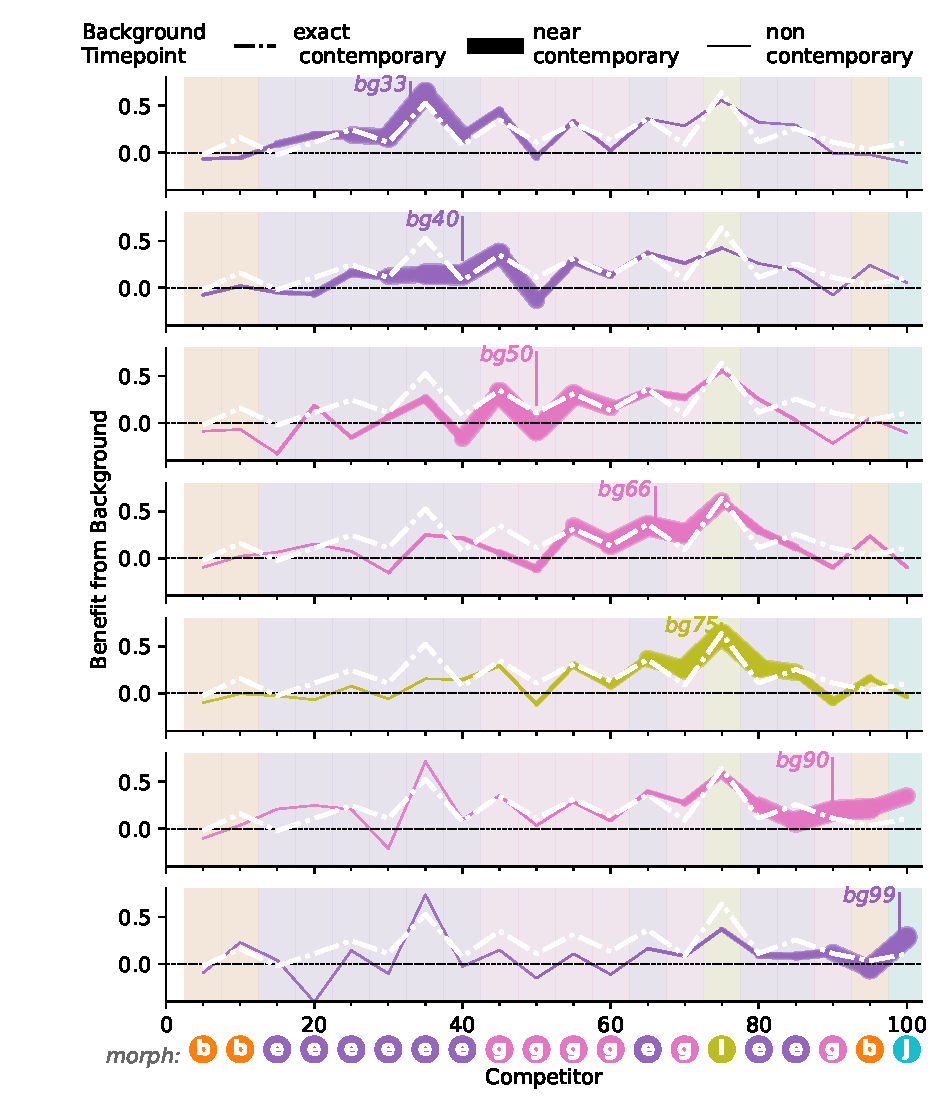
\includegraphics[width=\linewidth]{binder-2025-11-25-external-selfbb-timeshift.ipynb/binder/teeplots/2025-11-25-external-timeshift/viz=subplots+ext=.pdf}
\caption{TODO}
\end{subfigure}

\begin{subfigure}{\linewidth}

\includegraphics[width=\linewidth]{binder-2025-11-25-external-selfbb-timeshift.ipynb/binder/teeplots/2025-11-25-external-timeshift/hue=isexact+orient=h+viz=swarmplot+x=focal-prevalence+y=isexact+ext=.pdf%
}
\caption{TODO}
\end{subfigure}

\caption{%
\textbf{TODO.}
\footnotesize
TODO.
}
\label{fig:timeshift}

\end{figure}


Having identified that, within environmental context shaped by its cigar-like morphology, the case study strain gained a competitive advantage against other strains, we next sought to assess whether this niche construction effect produced ongoing self-acting selection.
Such selection, were it to have occurred, could then be tested for connections to evolved complexity.

To detect self-acting selection, we tested whether the case study strain exhibited ongoing adaptation to track changes in its own self context.
For this purpose, we repeated competitions against our ``measuring stick'' of cross-replicate comparators.
However, for these new assays, we time-shifted self context.
That is, competitions used background context from case study samples drawn at alternate timepoints --- rather than contemporary self-context.

Compared to time-shifted context, contemporary self-context provided substantially greater fitness benefit (Mann-Whitney test, $p<10^{-5}$, Cliff's $\delta=0.45$; Figure \ref{fig:timeshift}).
Nonetheless, time-shifted backgrounds still provided some benefit in 78 of 98 tested cases.
% --- including long temporal offsets of up to 50 transfer rounds (Supplementary Figure \ref{fig:timeshift-supp}).
Thus, while the underlying mechanism of niche construction appears to have remained generally stable, traits responsible for exploiting this niche indeed adapted over time to track changes in self-context.

\subsection{Self-acting Selection Maintains Complexity in Case Study Strain}
\label{sec:self-acting-selection-maintains-complexity-in-case-study-strain}

\begin{figure}

\begin{subfigure}{\linewidth}
\centering
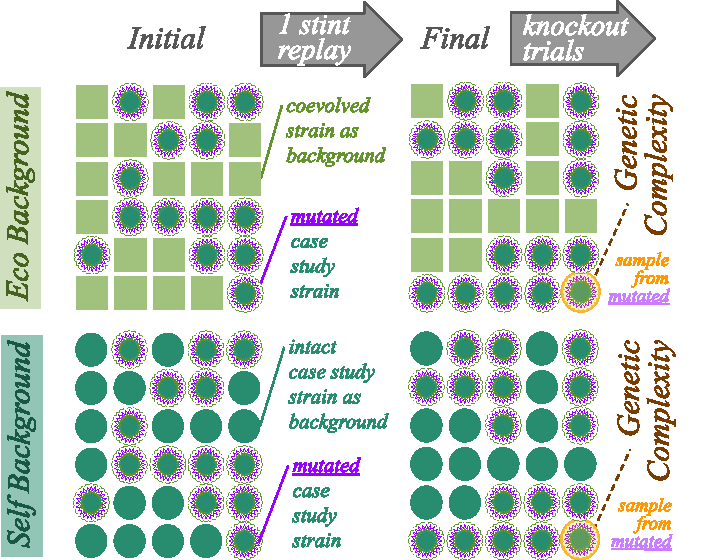
\includegraphics[width=0.85\linewidth]{img/mutagenized-replay-schematic.pdf}
~~

\caption{%
\footnotesize
replay trial design
}
\label{fig:replay-background:design}
\end{subfigure}

% The phenotype panel's teeplot PDF is emitted on a landscape page with its
% content laid a quarter turn over (its PNG twin is upright), so it is turned
% back upright here.
% Note that `angle' is given before `height' so that the height applies to the
% graphic as rotated, not as stored.
\begin{subfigure}{0.22\linewidth}
\centering

\includegraphics[angle=90,height=1.22in]{../binder/binder-2026-09-01-replay-phenotypes.ipynb/binder/teeplots/2026-09-01-replay-phenotypes/hue=source+viz=pointplot+y=prop+ext=.pdf}
\end{subfigure}%
\begin{subfigure}{0.18\linewidth}
\centering

\includegraphics[height=1.22in,trim=0 0 4cm 0,clip]{../binder/binder-2025-11-26-replaysmutagenized50.ipynb/binder/teeplots/2025-11-26-replaysmutagenized50/clip=62+hue=bucket+inner=quart+viz=violinplot+x=bucket+y=is-less-fit+ext=.pdf}
\end{subfigure}%
\begin{subfigure}{0.30\linewidth}
\centering

\includegraphics[height=1.22in,trim=2cm 0 0 0,clip]{../binder/binder-2025-11-23-replaysmutagenized08.ipynb/binder/teeplots/2025-11-23-replaysmutagenized08/hue=bucket+inner=quart+viz=violinplot+x=bucket+y=is-less-fit+ext=.pdf}
\end{subfigure}%
\begin{subfigure}{0.30\linewidth}
\centering

\includegraphics[height=1.22in,trim=2.5cm 0 0 0,clip]{../binder/binder-2025-11-26-replaysmutagenized50.ipynb/binder/teeplots/2025-11-26-replaysmutagenized50/clip=62+hue=bucket+inner=quart+viz=violinplot+x=bucket+y=is-less-fit+ext=.pdf}
\end{subfigure}

\vspace{-0.75ex}
\begin{subfigure}{0.70\linewidth}
\footnotesize
\caption{8 mutation dose}
\label{fig:replay-background:moderatedose}
\end{subfigure}%
\begin{subfigure}{0.30\linewidth}
\footnotesize
\caption{50 mutation dose}
\label{fig:replay-background:highdose}
\end{subfigure}

\vspace{-2ex}
\caption{%
\textbf{Constructed niche selects to maintain genotype complexity.}
\footnotesize
We performed short one-round replay trials on the case study strain, in either co-evolved or self context.
To enhance standing variation and weaken inherent self-context effects, replay genomes were subject to moderate mutagenesis --- dosed to maintain some functionally intact genomes (\ref{fig:replay-background:design}).
Replays in self context maintained higher genotype complexity than co-evolved context (Mann-Whitney test, \ref{fig:replay-background:moderatedose}).
Self context likewise better preserved the case study strain's cigar-like morphology --- recovered from 51 of 69 replays, versus 29 of 69 under co-evolved context (risk ratio 1.76, Fisher's exact test; leftmost panel of \ref{fig:replay-background:moderatedose}).
By contrast, more intense mutagenesis did not reproduce this effect, suggesting specificity to preserve already-evolved complexity (Mann-Whitney test, \ref{fig:replay-background:highdose}\protect\footnotemark).
Supplementary Figure \ref{fig:replay-background-early} shows replay results for transfer rounds 0 to 34.
}
\label{fig:replay-background}

\end{figure}

% adapted from https://tex.stackexchange.com/a/67030
\footnotetext{%
For legibility, Figure \ref{fig:replay-background:highdose} clips an extreme outlier with 142-site genotype complexity observed from self-context replay (Supplementary Figure \ref{fig:replay-background-outlier}).
}


Seeing evidence that the case study lineage's biogenic structure exerted self-acting selection, we next turned to test whether this selection stabilized its complexity.
To address this question, we carried out evolutionary replay trials, comparing complexity outcomes with and without self-context.

A practical challenge presents itself, however, in the task of removing --- or at least meaningfully abating --- self-context.
This problem is nontrivial, because any amount of the case study strain inherently introduces some degree of self-context.
To overcome this challenge, we mutationally attenuated the case study strain when seeding replay trials.
Mutagenic dose (8 mutations) was chosen such that most, but not all, seeded genomes were substantially disrupted.
As an additional benefit, applying mutation also enhanced standing variation --- improving sensitivity to detect selection on complexity.
% providing sufficient sensitivity to allow short 1-round replays.

Replays were compared between both a ``self context'' treatment and a ``co-evolved context'' treatment, with background context differing as intact case study lineage genomes or co-evolved lineage genomes (Figure \ref{fig:replay-background:design}).
To target the complexity maintenance period identified by split regression analysis, replays were conducted from transfer round 33 onwards --- thus, providing a sample of 67 single-round replays per treatment.
Endpoint complexity was measured on a surviving descendant of the mutagenized case study inoculum.

Across replays, intact self context preserved higher genotype complexity than co-evolved ecological context
(Mann-Whitney test, $p < 0.01$, $\delta = 0.25$; Figure \ref{fig:replay-background:moderatedose}).
Thus, biotic selection exerted by the case study strain indeed acted to stabilize its own complexity.

As a control experiment, we repeated replay experiments with a higher dose of 50 mutations --- sufficient to ensure substantial disruption to all seeded genomes.
% applied to seeded case study strain genotypes.
Under these conditions, complexity outcomes were indistinguishable between intact-self and co-evolved context treatments (Figure \ref{fig:replay-background:highdose}).
Thus, the case study strain's biotic selection appears to act specifically in maintaining its own evolved complexity.
In other words, evolved traits act to ``lock in'' complexity, as opposed to simply cultivating generic conditions conducive to complexity (e.g., weakening selection).

% We measured genetic complexity as our response variable.
% Having seen correlation between change in genetic complexity and phenotypic complexity in the case study strain, and as a more stable and sensitive measure of complexity, for these purposes we.

\subsection{Biotic Selection Drives Multicell Complexity}
\label{sec:biotic-selection-drives-multicell-complexity}

\begin{figure}

\begin{subfigure}[t]{0.41\linewidth}
\centering
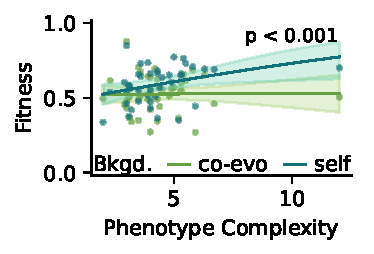
\includegraphics[width=\linewidth]{binder-2026-07-06-pcomplexity-gee.ipynb/binder/teeplots/2026-07-06-pcomplexity-gee/other=co-evo+viz=subplots+what=base+ext=.pdf}
\end{subfigure}%
\begin{subfigure}[t]{0.59\linewidth}
\centering
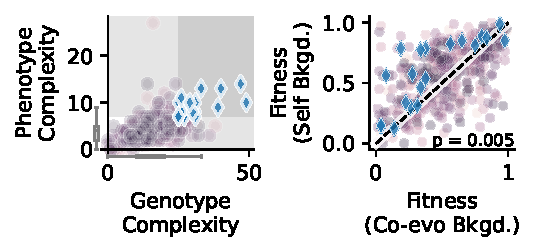
\includegraphics[width=\linewidth,trim={0.25cm 0 0 0},clip]{binder-2026-07-25-ecoselfcontext-pgcomplex-screen.ipynb/binder/teeplots/2026-07-25-ecoselfcontext-pgcomplex-screen/inner=box+iqr=shade+n=20+viz=subplots+ext=.pdf}
\end{subfigure}

\vspace{-4ex}

\begin{subfigure}[t]{0.37\linewidth}
\centering
\caption{\footnotesize niche construction selects for complexity }
\label{fig:general:gee-base}
\end{subfigure}%
\begin{subfigure}[t]{0.06\linewidth}
~
\end{subfigure}%
\begin{subfigure}[t]{0.57\linewidth}
\centering
\caption{\footnotesize niche construction is common in high-complexity strains }
\label{fig:general:pgcomplex-ecoself}
\end{subfigure}

% https://github.com/mmore500/oee4/blob/fa16a472ad6ac584ad7a5da7b7662729342ebc3b/binder/2026-07-25-ecoselfcontext-pgcomplex-screen.ipynb
% https://github.com/mmore500/oee4/blob/079d63f5e1583d71269a36cf9598431e4e34ac5e/binder/2026-07-06-pcomplexity-gee.ipynb
\caption{%
\textbf{Niche construction drives evolution of complexity across replicates.}
\footnotesize
Across original 100-stint replicates ($n=40$), fitness advantage of evolved complexity depends on self-acting selection (GEE, interaction coef. 0.145, $p < 0.001$; panel \ref{fig:general:gee-base}).
This relationship remains consistent after excluding case study strain (GEE, $p = 0.003$; Supplementary Figure \ref{TODO}) or disaggregating per-replicate point-in-time samples within replicates (autoregressive GEE; $p = 0.014$; Supplementary Figure \ref{TODO}).
Across additional 20-stint replicates ($n=400$), high-complexity replicates (top 5\% by genotype/phenotype complexity joint exceedance) disproportionately involve niche construction (Fisher's exact test, 18/2 vs. 216/164; $p = 0.004$); panel \ref{fig:general:pgcomplex-ecoself}).
This relationship remains consistent at 2.5\% and 7.5\% thresholds (9/1 vs. 225/165, $p=0.056$; 28/5 vs. 206/161, $p = 0.001$).
High-complexity replicates exhibit diverse morphologies, most differing from cigar morphology of case study (17/20; \url{https://hopth.ru/gz}).
}
\label{fig:general}
\end{figure}

\begin{figure}
\centering
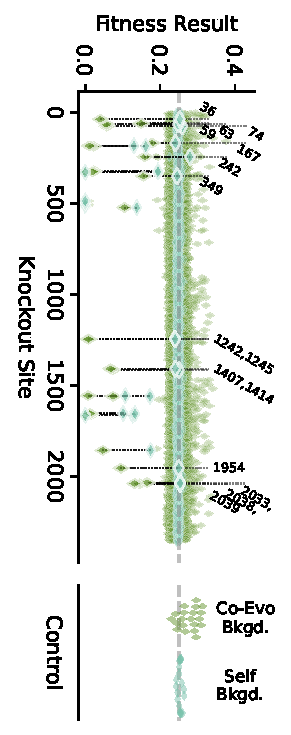
\includegraphics[height=0.9\linewidth,angle=90]{binder-2026-06-22-eco-gwas.ipynb/binder/teeplots/viz=subplots+ext=.pdf}

\vspace{-2ex}

% https://github.com/mmore500/oee4/blob/4a76b3624f7723879530f9b48310c96f8bc68b2a/binder/2026-06-22-eco-gwas.ipynb
\caption{%
\textbf{Case study strain selects for genotype complexity in co-evolved partner.}
\footnotesize
In stint-100 isolate of case study background strain, 14 genome sites exhibited strong adaptive benefit compared to single-site knockouts when tested with case study strain absent.
However, with case study strain present, adaptive benefit was detected at an additional 18 genome sites.
Co-evolutionary adaptation to case study strain thus accounts for 56\% (18/32) of detected genotype complexity in background strain.
}
\label{fig:general-supp:gwas}
\end{figure}


Having found biotic selection to stabilize evolved complexity on the case study lineage, we next sought to assess whether this pattern generalized more broadly across replicates.

To test whether analogous niche construction effects arose at all in other replicates, we screened for self-adaptation --- competitive advantage against cross-replicate comparators in self-dense biotic context.
Such self-adaptation arose repeatedly, with evidence in at least 10/39 additional lineages (Mann-Whitney tests, $\alpha = 0.05$; Supplementary Figures \labelcref{fig:external-bb-all,fig:general-supp:eco-vs-self}).

Seeing it did arise, we next tested whether self-adaptation influenced evolved complexity.
To sidestep wide variation in genome size after 100 transfer rounds, we compared across replicates using phenotype complexity --- how many distinct cell I/O operations contribute to strain fitness, reflecting the richness of evolved cell-cell interactions.
Where self-adaptation acts to maintain complexity, we would expect fitness under self-context and co-evolved context to diverge with complexity.
Comparing these fitness measures across our original $n=40$ replicates, we indeed found a stronger relationship between complexity and self-context fitness (binomial GEE, $p < 0.001$; $p = 0.003$ excluding case study replicate; Figure \ref{fig:general:gee-base}).
Further regression analysis confirms a direct relationship between self-adaptation and phenotype complexity (Supplementary Figure \ref{fig:TODO}).
Interestingly, no such relationship arose between fitness and phenotype complexity (Supplementary Figures \labelcref{fig:complexity-fitness-correlation-genetic-9s:phenotype-unagg,fig:complexity-fitness-correlation-genetic-9s:phenotype-agg,fig:complexity-fitness-correlation-genetic:phenotype-unagg,fig:complexity-fitness-correlation-genetic:phenotype-agg}).

Next, we sought to directly test whether highest-complexity multicell strains, such as the case study, rely on niche construction feedbacks.
For this purpose, we screened 400 additional 20-round trials, isolating the 20 most complex outcomes (top 5\%) by joint exceedance in genotype and phenotype complexity (Figure \ref{fig:general:pgcomplex-ecoself}, left).
Compared to lower-complexity strains, more high-complexity strains gained competitive advantage in self-dense contexts, consistent with niche construction effects.
In contrast to 85\% of high-complexity strains, only 54\% of lower-complexity strains gained such self-advantage (Fisher's exact test, $p = 0.005$, RR 1.58; Figure \ref{fig:general:pgcomplex-ecoself}, right).

% 17028, 21036, 28020
Among screened high-complexity strains, only 3 of 20 exhibit cigar-like morphologies analogous to the case study strain.
Thus, while the case study's evolutionary trajectory appears qualitatively reproducible, it only accounts for a small fraction of possible high-complexity outcomes --- nearly all alternate morphologies exhibit niche construction effects (16/17 vs. 204/380; Fisher's exact test, $p = 0.001$, RR 1.75).
Biotic selection on complexity thus appears to act more generally beyond the specific mechanism arising in our case study.
% Thus, the mechanism of self-acting selection appears more general than one particular life history.

\subsection{Biotic Selection Acts Between Co-evolving Lineages}
\label{sec:biotic-selection-acts-between-coevolving-lineages}

\begin{figure}
\centering

\begin{subfigure}{\linewidth}
\centering
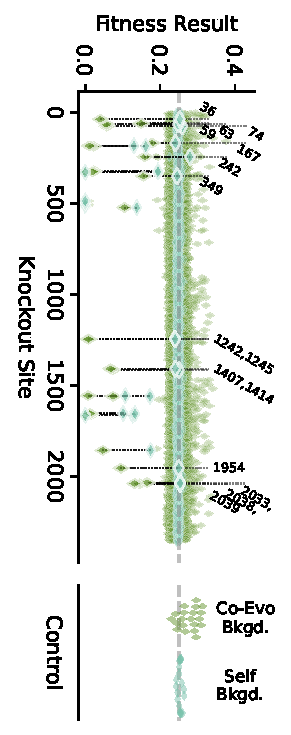
\includegraphics[height=0.9\linewidth,angle=90]{binder-2026-06-22-eco-gwas.ipynb/binder/teeplots/viz=subplots+ext=.pdf}

\caption{\footnotesize TODO}
\label{fig:ecogwas:sites}
\end{subfigure}

\vspace{1ex}

\begin{subfigure}{\linewidth}
\centering

\includegraphics[height=0.35\linewidth]{binder-2026-08-13-eco-gwas-weakstrong.ipynb/binder/teeplots/2026-08-13-eco-gwas-weakstrong/col=classification+hue=classification+style=classification+viz=relplot+x=focal-prevalence-backgroundbb+y=focal-prevalence-focalbb+ythresh=0.45+ext=.pdf}%

\includegraphics[height=0.35\linewidth]{binder-2026-08-13-eco-gwas-weakstrong.ipynb/binder/teeplots/2026-08-13-eco-gwas-weakstrong/color=white+viz=boxplot+x=classification+y=count+ythresh=0.45+ext=.pdf}

\caption{\footnotesize TODO}
\label{fig:ecogwas:ythresh045}
\end{subfigure}

% https://github.com/mmore500/oee4/blob/34f2116c799c849f329e91f544e57daa23eff9da/binder/2026-06-22-eco-gwas.ipynb
% https://github.com/mmore500/oee4/blob/34f2116c799c849f329e91f544e57daa23eff9da/binder/2026-08-13-eco-gwas-weakstrong.ipynb
\caption{%
\textbf{Case study strain selects for genotype complexity in co-evolved partner.}
\footnotesize
In stint-100 isolate of case study background strain, 14 genome sites exhibited strong adaptive benefit compared to single-site knockouts when tested with case study strain absent.
However, with case study strain present, adaptive benefit was detected at an additional 18 genome sites.
Co-evolutionary adaptation to case study strain thus accounts for 56\% (18/32) of detected genotype complexity in background strain.
TODO
}
\label{fig:ecogwas}
\end{figure}


In addition to conspecific peers, natural multicells encounter numerous heterospecific biota from co-evolving lineages.
To assess the role of such broader interactions in the evolutionary origins of multicell complexity, we next investigated how selection between co-evolving lineages can produce evolved complexity.

Recall, as noted earlier, that the case study strain and its co-evolved partner both adapted to each other, exhibiting competitive advantage in co-evolved context (Supplementary Figure \ref{fig:external-bb-reciporical}).
Thus, to begin, we examined whether --- in addition to selecting on itself --- the case study strain selected for genotype complexity in its co-evolved ``background'' partner.
Under self-context conditions, single-site knockout trials identified 17 sites as adaptive (Figure \ref{fig:ecogwas:sites}).

These 17 identified sites remained adaptive when tested in the presence of the case study strain, rather than self-context conditions.
However, in addition, competition experiments identified 15 further sites adaptive exclusively in the presence of the case study strain.
Thus, in this case, co-evolutionary interactions with the case study strain substantially drove evolved complexity in its co-evolved partner --- among 32 adaptive sites, 47\% arose by biotic selection between lineages.

Having found that co-evolutionary interactions drove complexity in the case study's co-evolved partner, we next sought to assess whether biotic selection between lineages produced genotype complexity more broadly.
For this purpose, we surveyed our 400 additional 20-round trials to sample replicates with weak co-evolutionary adaptation, and compared them to replicates with strong co-evolutionary adaptation --- measured by competitive advantage specific to co-evolved context.
Among sampled strains, adaptive sites specific to co-evolved context were detected in 6 of 7 exhibiting strong co-evolutionary adaptation --- more than 2 of 7 detected under weak co-evolutionary adaptation (Mann-Whitney U test; $p=0.016$, Cliff's $\delta=0.75$; Figure \ref{fig:ecogwas:ythresh045}).
Thus, partner-specific selection appears to have additionally acted in creating evolved genotype complexity.
Taken together, these results implicate biotic selection in general --- self-generated and co-evolved alike --- as a key driver of multicellular complexity.
